
\begin{frame}{Contents}
   \begin{itemize}
       \item[\textcolor{red}{$\rhd$}] Chisel の導入
       \item Pros. \& Cons.
       \item ChiselImProc の説明
       \item Vivado HLS との比較
   \end{itemize} 
\end{frame}


\begin{frame}{Chisel の導入}
    \begin{itemize}
        \item JDK とsbt を導入 \\
            (\url{https://www.scala-sbt.org/})
        \item chisel-template をclone \\
            (\url{https://github.com/freechipsproject/chisel-template})
            
        \item プロジェクト名をリネーム
    \end{itemize}
    
\end{frame}

\begin{frame}[fragile]{Chisel の文法}

    \begin{itemize}
        \item 各モジュールはModuleクラスを拡張して作成。
        \begin{lstlisting}[language=Scala,caption={Lチカモジュール}]
class Hello extends Module {
     val io = IO(new Bundle {
        val led = Output (UInt (1.W))
     })
     val CNT_MAX = (50000000 / 2 - 1).U;
     
     val cntReg = RegInit(0.U(32.W))
     val blkReg = RegInit(0.U(1.W))
     
     cntReg := cntReg + 1.U
     when (cntReg === CNT_MAX) {
        cntReg := 0.U
        blkReg := ~blkReg
     }
     io.led := blkReg
}
        \end{lstlisting}
    \end{itemize}
    
\end{frame}



\begin{frame}[fragile]{信号型と定数}
    \begin{itemize}
        \item ビットのベクトルを表す3つのデータ型。
            \begin{lstlisting}
Bits(8.W)
UInt(8.W)
SIng(8.W)
            \end{lstlisting}
        \item データ幅はWidth型で表す。
        \item 定数データを記述するときはメソッド呼び出しを用いる。
            \begin{lstlisting}
8.U(4.W)    // ビット幅は引数で指定
0.U
-3.S        // ビット幅は指定しなくても推論してくれる
            \end{lstlisting}
        \item 論理型(UInt(1.W)の拡張)
            \begin{lstlisting}
Bool()
true.B
false.B
            \end{lstlisting}
    \end{itemize} 
\end{frame}


\begin{frame}[fragile]{組み合わせ回路}
   \begin{itemize}
       \item 論理演算子
       \begin{lstlisting}
val and = a & b    // bitwise and
val or = a | b     // bitwise or
val xor = a ^ b    // bitwise xor
val not = ~a       // bitwise negation
       \end{lstlisting}
       
       \item 算術演算子
       \begin{lstlisting}
val add = a + b
val sub = a - b
val neg = - a
val mul = a * b
val div = a / b
val mod = a % b
       \end{lstlisting}
   \end{itemize} 
\end{frame}



\begin{frame}[fragile]{組み合わせ回路}
    \begin{itemize}
        \item 信号タイプを先に定義してから、更新演算子を使用して
        信号に値を割り当てることもできる。
        \begin{lstlisting}
val w = Wire (UInt())
w := a & b
        \end{lstlisting}
        
        \item 1ビットの抽出
        \begin{lstlisting}
val sign = x(31)
        \end{lstlisting}
        
        \item 範囲指定で抜き出し
        \begin{lstlisting}
val lowByte = largeWord(7, 0)
        \end{lstlisting}
        
        \item 信号の結合
        \begin{lstlisting}
val word = Cat(highByte, lowByte)
        \end{lstlisting}
    \end{itemize}
\end{frame}



\begin{frame}[fragile]{組み合わせ回路}
    \begin{itemize}
        \item マルチプレクサ
        \begin{lstlisting}
val y = Mux (sel, a, b)
        \end{lstlisting}
        \begin{figure}[h]
            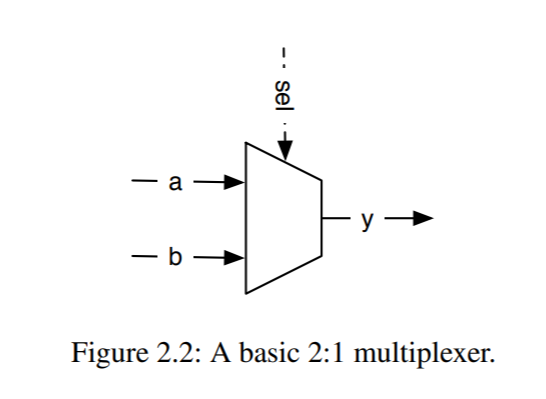
\includegraphics[width=0.5\textwidth]{./figures/mux.png}
        \end{figure}
    \end{itemize}
\end{frame}



\begin{frame}[fragile]{レジスタ}
    \begin{itemize}
        \item リセット時に0で初期化される8ビットレジスタ
        \begin{lstlisting}
val reg = RegInit(0.U(8.W))
reg := d                    // 更新演算子で更新
val q = reg                 // レジスタの値を取り出す
        \end{lstlisting}
        
        \item 初期値が不定(X)のレジスタ
        \begin{lstlisting}
val reg = Reg(UInt(8.W))
        \end{lstlisting}
        
        \item カウンター
        \begin{lstlisting}
val cntReg = RegInit(0.U(8.W))
cntReg := Mux (cntReg === 9.U, 0.U, cntReg + 1.U)
        \end{lstlisting}
    \end{itemize}
    
\end{frame}



\begin{frame}[fragile]{Bundle と Vec}
    \begin{itemize}
        \item Bundle: 異なるタイプの複数の信号をまとめる。
        \begin{lstlisting}
class Channel() extends Bundle {
    val data = UInt(32.W)
    val valid = Bool()
}
        \end{lstlisting}
        
        \item フィールドにはドット表記でアクセス。
        \begin{lstlisting}
val ch = Wire (new Channel())
ch.data := 123.U            // 更新演算子で更新できる
ch.valid := true.B          // 更新演算子で更新できる
val b = ch.valid            // フィールドだけを参照
val channel = ch            // 全体を参照
        \end{lstlisting}
        
        \item Vec: 同じタイプの複数の信号をまとめる。
        \begin{lstlisting}
val v = Wire (Vec (3, UInt(4.W)))
v(0) := 1.U                 // アクセスは配列と同じ
v(1) := 3.U                 // アクセスは配列と同じ
v(2) := 5.U                 // アクセスは配列と同じ
        \end{lstlisting}
    \end{itemize}
    
\end{frame}




\begin{frame}[fragile]{テスト}
    PeekPokeTesterでIOポートからデータを入出力できる
    \begin{lstlisting}
class DeviceUnderTest extends Module {
    val io = IO (new Bundle {
        val a = Input (UInt(32.W))
        val b = Input (UInt(32.W))
        val out = Output (UInt(2.W))
    })
    io.out := io.a & io.b
}
    \end{lstlisting}
    
    \begin{lstlisting}
class TesterSimple (dut: DeviceUnderTest) 
        extends PeekPokeTester(dut) {
    poke (dut.io.a, 0.U)
    poke (dut.io.b, 1.U)
    step (1)
    println ("Result is: " + peek(dut.io.out).toString)
    poke (dut.io.a, 4.U)
    poke (dut.io.b, 2.U)
    step (1)
    expect (dut.io.out, 0)
}
    \end{lstlisting}

    
\end{frame}

